\documentclass[11pt,a4paper]{article}

% Packages
\usepackage[a4paper,margin=1in]{geometry}   % sane margins
\usepackage[utf8]{inputenc}
\usepackage[T1]{fontenc}
\usepackage{amsmath,amssymb}                % math
\usepackage{graphicx}                       % figures
\usepackage{booktabs}                       % nice tables (\toprule etc.)
\usepackage{caption}
\usepackage[labelfont=bf,font=small]{caption}
\usepackage[table]{xcolor}
\usepackage{hyperref}                       % clickable refs/links
\hypersetup{colorlinks=true, linkcolor=blue, citecolor=blue, urlcolor=blue}
\usepackage[capitalise]{cleveref}           % \cref{} for smart cross-refs
\usepackage[round,authoryear]{natbib}       % (Author, Year) citations
\usepackage{setspace}
\setstretch{1.08}                           % slightly open leading, still compact
\usepackage{titlesec}
\titlespacing*{\section}{0pt}{1.4em}{0.7em}
\titlespacing*{\subsection}{0pt}{1.1em}{0.5em}

% Title
\title{
    \vspace{-1em}
    A Short Report on Simulation Based Inference\\[0.4em]
    \large Scientific Machine Learning Seminar}
\author{
  Jakob Dammann\\
  \small Faculty of Physics and Astronomy, University Heidelberg\\
  \small \texttt{jakob.dammann@stud.uni-heidelberg.de}\\[0.3em]
  \small Supervisor: Tobias Buck\\
  \small Interdisciplinary Center for Scientific Computing, University Heidelberg
}
\date{\today}

\begin{document}

\maketitle

% ---------------------------------------------------------------------
\begin{abstract}
\noindent
Simulation Based Inference (SBI) offers a novel approach to solve inverse problems powered by machine learning. 
Hereby, a neural network learns to relate datapoints from a simulated dataset to a posterior distribution of model parameters.
It can outperform classical Bayesian inference methods in inference speed and posterior accuracy.
Additionally, SBI does not require any likelihood evaluation which often is computationally costly or has to be approximated.
Common problems like model misspecification, neural inaccuracies or miscalibrated posteriors can limit the usefulness of SBI if they are not circumvented.
Exemplary usecases for SBI are inferring the complex parameter posteriors from planetary microlensing events or gravitational waves from black hole mergers.
\end{abstract}

% Sections
% ---------------------------------------------------------------------
\section{Introduction}%
\label{sec:intro}

% What are inverse problems (in contrast to forward problems)
In computational physics there are usually two types of problems to solve: 
Firstly, forward problems where the parameters and/or boundary conditions of a model are given and the goal is to find data or a data distribution which adheres to this model. 
For example in the case of given parameters and initial values this is a typical simulation.

Though secondly, there are also inverse problems where the data is the preset and now the parameters or parameter distributions of the assumed model have to be inferred.
So here the data likely comes from an observation and the parameters which represent physical properties of the system have to be computed.
This is the type of problem that will be explored in this review.

% Inferring the parameter posterior with classical Bayesian methods or Simulation Based Inference
A rather simple case of solving an inverse problem is the use of linear regression to fit a function to a given dataset.
But for more complex models also methods with higher efficiency are needed.
The classical approach here is to use Bayesian methods to infer the parameter posterior distribution, but Simulation-Based Inference introduces machine learning techniques to solving inverse problems.
SBI is able to solve these problems in some cases more efficiently and computationally cheaper.
% Short: examples where posterior estimation is needed
Applications where SBI shows advantages are (but not limited to) gravitational microlensing \citep{microlensing-sbi}, gravitational wave physics \citep{flow-matching-sbi} and neuroscience \citep[Sec.\,4.3]{sbi-guide}.

% Section Roadmap
In \cref{sec:bayes} the general concepts of classical Bayesian inference are first explored, specifically focussing on Markov-Chain-Monte-Carlo methods.
Then SBI and its underlying concepts are introduced in \cref{sec:sbi} and exemplified in \cref{sec:example} with the help of a toy-example.
The advantages and limitations of SBI are presented in \cref{sec:benefits-limitations}.
Two exemplary applications with results are portrayed in \cref{sec:application} and a conclusion is given in \cref{sec:conclusion}.


% ---------------------------------------------------------------------
\section{Classical Bayesian Inference}%
\label{sec:bayes}

% General concept of Bayes equation
The most outstanding feature of Bayesian Inference in comparison to regression is that the output of BI is a posterior distribution of the parameters instead of just a likely parameter set from this distribution.
So instead of just computing $\theta \sim p(\theta|x)$, the result is the full $p(\theta|x)$ distribution.
The naming convention here is that $\theta$ is the set of parameters from the model and $x$ is the observed data. 

The underlying concept is the Bayes equation 
\begin{equation}
  p(\theta|x) = \frac{p(x|\theta)}{p(x)} p(\theta)
  \label{eq:bayes}
\end{equation}
from Bayesian statistics where $p(\theta|x)$ is the posterior distribution, $p(x|\theta)$ the likelihood, $p(x)$ the evidence and $p(\theta)$ the prior distribution.
While the prior can be chosen adequately according to assumed distributions of the model parameters and the evidence is just a normalizing factor, the likelihood $p(x|\theta)$ has to somehow be calculated, evaluated or approximated in numerical methods of inferencing the posterior.
This is the most important and also most costly step of classical Bayesian Inference \citep[Sec.\,1]{sbi-guide}.

% Methods of inference, MCMC
Different methods of Bayesian inference solve this in different ways.
Markov chain Monte Carlo (MCMC) methods are relatively simple and widely used for inferring posteriors.
These evaluate the likelihood many times randomly in the parameters space and build a posterior distribution from that.
In Metropolis-Hastings, a MCMC method, the prior and likelihood value at a random point in the parameter space determines if this point is accepted or rejected.
The accumulated distribution of the accepted points then converges to the posterior after many evaluations \citep{Hastings1970}.

% Limitations: convergence, local approximation, multimodal posteriors
There are adjusted methods that can make the algorithm more efficient (like introducing random walk instead of true random sampling) but all classical Bayesian inference methods suffer from similar key limitations:
The convergence to a posterior that is accurate enough for the specific application takes many evaluations of the likelihood and is therefore very computationally expensive.
For the applications that are later shown in \cref{sec:application} this can be up to 1 second per evaluation, for an adequately sampled posterior distribution the computation time per analyzed dataset can be huge.

In complex models the exact evaluation of the likelihood is often not possible or a lot more computationally expensive, so it has to be approximated by a Gaussian distribution, usually as part of the $\chi^2$ method.
This inserts another error source into the posterior distribution.

Classical Bayesian inference methods also have the problem that they cannot model multimodal posteriors very well.
The algorithm often gets stuck in one mode and is unable to jump to another, this becomes a problem in models with a lot of close degeneracies \citep[Sec.\,1,\,2.1]{sbi-guide}.
In turn, grid searches and human intervention are often needed which increases the time and effort of the data analysis process.
This may not be a possibility for the huge amounts of data that needs to be processed in modern science.


% ---------------------------------------------------------------------
\section{Introduction to Simulation-Based Inference}%
\label{sec:sbi}

% Skip Likelihood evaluation, implicit in simulation
The key feature of Simulation-Based Inference is the skipping of the computationally expensive likelihood evaluation.
This is the reason SBI is sometimes also called Likelihood-Free Inference.
Instead of explicitly using a method to evaluate the likelihood at specific points in parameter space, the likelihood is implicitly given when sampling data from a simulator of the model.
A neural network will train on this simulated dataset to infer a parameter posterior distribution from an observation.
The likelihood still exists inside the dataset but does not have to be calculated or approximated.

% Neural Posterior Estimation (NPE)
This review focusses on the direct inference of posteriors, this methodology is called Neural Posterior Estimation (NPE).
This is in contrast to Neural Likelihood Estimation (NLE) and Neural (Likelihood-)Ratio Estimation (NRE), they respectively require an additional step of computation to achieve the posterior but may offer advantages or more insight in the analysis process.

% Sampling from simulator, train neural network, estimate posterior from observation
The SBI workflow can be subdivided into three steps as shown in \cref{fig:sbi-workflow}:
First, the simulator has to generate a relatively large dataset in accordance with the physical model.
To achieve this, an adequate parameter prior distribution is chosen according to guesses on the physical properties of the model, e.g. the range of specific parameters.
The simulator then samples $x_i$ from the likelihood $p(x|\theta_i)$ and therefore generates a $(x_i,\theta_i)$ dataset.
The likelihood is implicitly contained in the dataset but because the simulation solves a forward problem, this step is not very computationally costly.

\begin{figure}
  \centering
  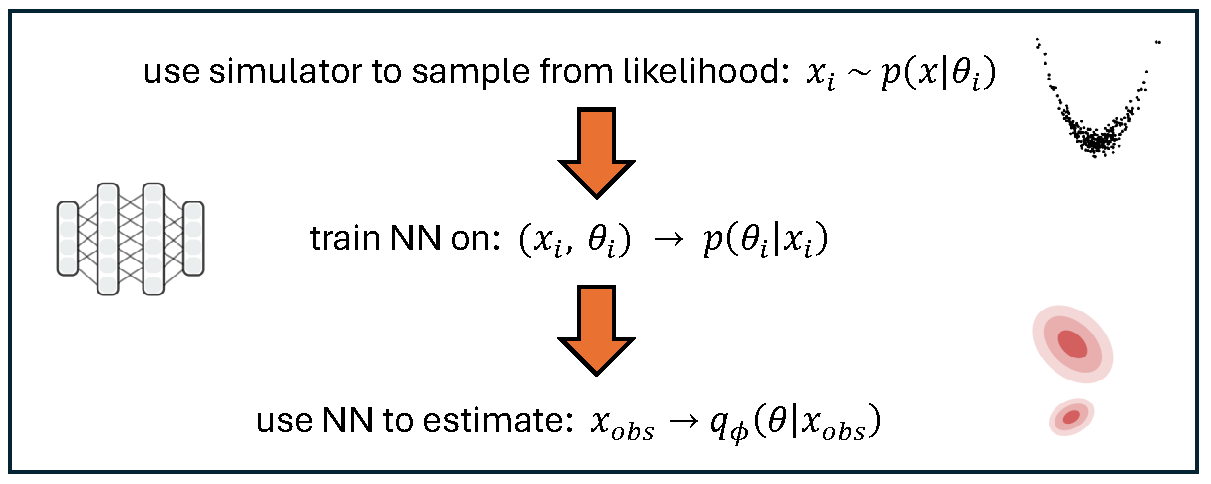
\includegraphics[width=0.8\linewidth]{figures/figure_sbi-workflow.pdf}
  \caption{Schematic overview of the SBI-workflow. Three steps are shown: simulation of a dataset $(\theta_i,x_i)$, training of the neural network (NN) to estimate the true posterior density $p(\theta_i,x_i)$ and posterior estimation which maps the observed data $x_\text{obs}$ to an estimated posterior distribution $q_\phi(\theta|x_\text{obs})$. Parts of the figure are adapted from \cite{sbi-guide}.}%
  \label{fig:sbi-workflow}
\end{figure}

Next, a neural network is trained to map each tuple $(x_i,\theta_i)$ to an estimated posterior density $q_\phi(\theta_i|x_i)$.
The network architecture can in theory be chosen freely but Normalizing Flows is commonly used.
The loss function
\begin{equation}
  \mathcal{L}(\phi) = \mathbb{E}_{(\theta_i,x_i) \sim p(\theta,x)}\!\left[-\log q_\phi(\theta_i|x_i)\right]
  \label{eq:loss}
\end{equation}
is minimized to improve the network weights.
It consists of the expectation value over all sampled tuples of the negative logarithm of the estimated posterior density.
This is very similar to the definition of a cross entropy and will result in a balancing act between low loss values and high confidence in the posterior.
Since the posterior has to be normalized, maximizing $q_\phi(\theta_i|x_i)$ at the correct $\theta_i$ has the drawback of having to be more confident by making the distribution more slim.
So the estimated posterior density $q_\phi(\theta_i|x_i)$ is trained towards representing the true posterior $p(\theta_i|x_i)$.

Lastly, the observed datapoint $x_\text{obs}$ is inserted into the network and evaluated inside an interval of $\theta$ at any resolution.
This will output the posterior distribution of any observation with relatively low computational cost.
It is worthy to note that there is no need for further training when analyzing new data under the assumption of the same model \citep[Sec.\,2.2,\,3]{sbi-guide}.


% ---------------------------------------------------------------------
\section{Simple SBI Example}%
\label{sec:example}

% Example: angled throw
A fairly simple demonstration of SBI is done in the following section with the help of the simulation of an angled throw.
The structure and code of this toy-example is adapted from \cite{sbi-guide}.

A ball is thrown from the origin at a specific angle $\theta$. 
This is the sole parameter of the model.
The ball lands on the ground at a specific distance from the origin, again this is the only data value $x$.
The system behaves according to the physical laws of gravity, the flight trajectory should be a parabola.
To turn the model probabilistic and make it harder for SBI to infer the posterior, a varying wind speed is added as a noise source.

Now it is not trivial to infer the posterior distribution of throwing angles from just a single distance measurement.
Even classical Bayesian methods would have problems since the posterior has two modes, a short throw could have come from either a very low angle or very high angle.
A few example trajectories are shown in \cref{fig:angled-throw}a.

\begin{figure}
  \centering
  % \includegraphics[width=0.8\linewidth]{figures/example.pdf}
  \fbox{\parbox[c][4cm][c]{0.8\linewidth}{\centering Figure placeholder}}
  \caption{Structure of SBI simulation and training for the simple example of an angled throw. Shown in a: simulation of throw trajectories, b: prior distribution of parameters $\theta_i$, c: simulated dataset $(\theta_i,x_i)$, d: training of the neural network to map $(\theta_i,x_i)$ to $q_\phi(\theta_i,x_i)$. Parts of the figure are adapted from \cite{sbi-guide}.}%
  \label{fig:angled-throw}
\end{figure}

% choose parameter prior, create simulator of throw, simulate dataset
A parameter prior for throwing angle $\theta$ also needs to be chosen, here a Gaussian distribution which is limited between $0^\circ$ and $90^\circ$ and has its maximum at $35^\circ$ (as shown in \cref{fig:angled-throw}b) is a logical choice.
Parameter values $\theta_i$ are sampled from this prior and put into the simulator that contains the probabilistic model of the angled throw as described above.
A lot of angle - distance tuples $(\theta_i,x_i)$ are created, building the dataset that is shown in \cref{fig:angled-throw}c.

% train neural network, here normalizing flows, any network works
This dataset is used to train a neural network based on the architecture of Normalizing Flows.
The input of the network will be a tuple $(\theta_i,x_i)$ while the output is a predicted posterior density value $q_\phi$ at specifically $\theta = \theta_i$ in the parameter space under the assumption $x = x_i$.
This is shown as a schematic in \cref{fig:angled-throw}d.
The network is optimized with the loss function in \cref{eq:loss} as explained in \cref{sec:sbi}.

% use network to evaluate observation, data and param interval
With the trained network a posterior distribution is generated by inputting the observation $x_\text{obs}$, for example $x_\text{obs} = 10\,\text{m}$ and sampling the posterior in an interval of angles $\theta$ values.
This is done for a few hypothetical observations and sampled for $0^\circ < \theta < 90^\circ$.
The sampling rate of $\theta$ can be chosen freely but affects the computational cost of the algorithm and may not offer any advantages when increasing it above a neural estimation accuracy.
Though in this very simple example the computational cost is negligible.
The results are shown in \cref{fig:angled-throw}e.
For smaller $x_\text{obs}$ the two modes in the posterior are easily visible as two separate peaks.

% ---------------------------------------------------------------------
\section{Benefits and Limitations}%
\label{sec:benefits-limitations}

SBI is able to outperform classical Bayesian Inference in specific contexts.
The method's benefits can be summarized into three main concepts that are presented in the following section along with their limitations.

% Likelihood-free (no approximation or expensive computation), 
First of all, the inference of the posterior is likelihood-free.
There is no need to explicitly evaluate the likelihood at random points in the parameter space like it is the case for MCMC, the likelihood is implicitly contained inside the dataset from the simulator the neural network is trained on.
That means the inference itself can be made a lot faster and there is no need for approximations of the likelihood in the process like it is often done for Bayesian Inference.

% very fast inference (Amortized Inference), 
Adjacent to that, SBI offers the concept of Amortized Inference.
Here the largest amount of computational cost is paid upfront when running the simulator and training the neural network, but the actual inference by the network is very fast and cheap.
This can speed up the analysis for research purposes a lot if a model is reused for a lot of data since there is no additional simulating and training needed after the weights for a network are optimized.
For complex models this is especially relevant, in classical Bayesian Inference a considerable amount of computation time would be needed at each likelihood evaluation.

% multimodal posteriors
And thirdly, SBI is able to model the multimodality of posteriors very well. 
It does not have to explore different modes manually like it is often the case for MCMC where the algorithm can get stuck inside a specific mode.
The neural network is aware of the entire posterior at once, not only dependent on a local likelihood approximation.

% Limitations: 
Though bundled with these advantages there are also limitations that exist in SBI algorithms.
% Upfront training, 
The previously mentioned upfront simulation and training due to Amortized Inference may be a drawback when there is only a limited amount of observations to be processed.
Therefore, the gain in inference speed is may not be worth it.

% model misspecification (common pitfall)
Since SBI is only as good as the simulator, a common pitfall is model misspecification.
When giving the neural network an observation that has not been simulated before, because such a case is not included in the model, the network will output a nonsensical posterior distribution that is not related to real physics.
To illustrate, when giving the trained network from the example in \cref{sec:example} a distance larger than any possible throw, the output will be an unpredictable posterior of angles that would never lead to such a distance.
In complex models this is not trivial to avoid.

% posterior is a neural estimation
It is important to remember that the output posterior is only a neural estimation and its quality depends on the simulations, the network architecture as well as training.
There is no convergence guarantee analogous to MCMC to assure that the estimated posterior is getting closer to the true posterior.
MCMC becomes asymptotically exact for long chains, but here the estimate is exact only in the limit of infinite training data and network capacity which makes the quality difficult to assess.

% uncalibrated posterior
A common problem of posteriors inferenced via NPE is that they may be miscalibrated.
They can have biases, meaning a shifted mean to either side, or are either over- or underconfident, resulting in a distribution that is spread out not enough over too much.
Though miscalibration can be diagnosed quite effectively with the help of quantile-occurence plots.
The posterior probability of the true value is compared with how often it actually occurs in a validation dataset and can therefore show errors in posterior accuracy on a global scale.
If miscalibration is hinted at in the quantile-occurence plots, changes to the network and training are probably necessary \citep[Sec\,1,\,2.2,\,3]{sbi-guide}.

% ---------------------------------------------------------------------
\section{Application}%
\label{sec:application}

% Short explanation of microlensing
The research area of gravitational microlensing is one of the prime examples where SBI shines in the data analysis pipeline.
When a star with an exoplanet in orbit moves into the line of sight between earth and a bright background star the light of background star is lensed around the foreground star and exoplanet and magnified in a very specific way.
This effect cannot be spatially resolved but telescopes can measure the change of brightness as a lightcurve.
The shape of the lightcurve is defined by the physical properties of both stars and exoplanet resulting in a large amount of parameters (around 11) and a complex model while the data is often limited.
Additionally, the model is also highly degenerate and often has multiple complex modes that have to explored manually when using classical Bayesian Inference.

% Results of usage of SBI \citep{microlensing-sbi}
This is the reason \cite{microlensing-sbi} is testing the capabilities of SBI for microlensing data from the Roman Space Telescope.
The training was done with a dataset of more than 275,000 simulated events and about 25 hours.
SBI was able to increase the computation speed drastically from $1$ simulation per second which would be needed for one MCMC step to $10^5$ posterior samples per second.
What was found is that all the posterior modes where accurately modeled though some biases existed in the posterior.
The authors recommend following up on SBI with MCMC to converge on an accurate posterior and also the most likely solution.
This demonstrates SBIs functionality in the data analysis pipeline for quickly exploring multimodality of posteriors and attaining initial values for further inference methods.

% Short explanation of gravitational waves and black hole mergers
Similarly, the models needed to analyze gravitational wave signals from black hole mergers are dependent on a lot of parameters but only very limited data is available.
% FMPE \citep{flow-matching-sbi}
\cite{flow-matching-sbi} use SBI in their data analysis pipeline for gravitational wave events but implement Flow Matching Posterior Estimation (FMPE) in their SBI architecture.
Instead of Normalizing Flows FMPE is based on a Flow Matching neural network. 
This learns a vector field transformation from a simple distribution to the real posterior and not the transformation of datapoints, achieving fewer parameters to describe the same transformation, a more expressive neural network and 30\% reduced training time.
In turn, the inference time is increased since the sampling also requires solving an ordinary differential equation dependent on the velocity field output.

% Other applications
Generally all physics or science research fields which are heavy in data processing would likely benefit from an implementation SBI in specific contexts.
Other fields of research noted in \cite{sbi-guide} for SBI applications are psychophysics and neuroscience.


% ---------------------------------------------------------------------
\section{Conclusion}%
\label{sec:conclusion}

% Benefits
Simulation-Based Inference offers benefits that are advantageous in specific parts of data analysis pipelines in many areas of physics.
Namely, these are the Likelihood-Freeness of the Method, Amortized Inference and the ability to accurately model multimodality in posteriors.
% Limitations
Limitations include the possibility of misspecification in the simulation, miscalibration of the posterior in the neural network and the neurally approximated nature of the output posterior.
These have to be looked out for and avoided by validation techniques like quantile-occurence plots.

% When to use SBI\: inverse problem, time critical inference, expensive likelihood evaluation, multimodal posterior
An ideal use case would for SBI would be an inverse problem where the inference is time-critical, a likelihood evaluation is expensive and the posterior is possibly multimodal.
In the data analysis pipeline SBI is very valuable to get a globally accurate estimation of the posterior. 
It can be used to explore the parameter space and can be refined by expensive classical Bayesian methods at specific very likely solutions like it was recommended by \cite{microlensing-sbi}.

% Conclusion
As datasets in physics or other sciences get larger, faster but still accurate ways of inferring information are needed and in that regard Simulation-Based Inference is going to be a very useful methodology for scientific data analysis based on machine learning.
An influx in the amount of use of SBI for physics in the next few years is likely.
Open challenges need to be addressed and improvements are still to be made but SBI will presumably grow into a key part of the modern Bayesian data analysis toolkit.



% TODO:
% add sections to SBI-guide citations
% figures
% change benefits position
% This


% ---------------------------------------------------------------------
\bibliographystyle{plainnat}
\bibliography{references}

% ---------------------------------------------------------------------
% \appendix
% \section{Additional Material}%
% \label{sec:appendix}
% Supplementary derivations, extra tables, or code listings.

\end{document}
